% !TEX root =  paper.tex
\section{Introduction}

One of the critical components of connectomics---the field concerned with reconstructing the wiring diagram of the brain at nanometer resolution---is automatic segmentation of electron microscopy (EM) images.
With recent advancements in EM acquisition techniques, neuroscientists can now generate a terabyte of image data every hour~\cite{richard2016imaging}.
These images are typically anisotropic with $4$nm resolution in the $xy$ plane and \numrange{30}{40}nm between slices. 
At this resolution, we can see the axon terminals and dendritic spines, and the synaptic connections between them.
Neuroscientists hope to further the understanding of the brain's underlying circuitry with accurate reconstructions of every neuron and classification of every synapse.


An ambitious manual reconstruction effort in the 1980s resulted in the first complete connectome of any animal, the \textit{Caenorhabditis elegans} worm~\cite{white1986structure}. 
This species has 302 neurons and manual labeling required several years.
More recent studies focus on \textit{Drosophila} flies~\cite{jovanic2016competitive,takemura2015synaptic},  rodents~\cite{richard2016imaging}, and even humans~\cite{sporns2005human}. 
With an EM throughput of one terabyte per hour, neuroscientists can image a cubic millimeter of data (two petabytes) in six months~\cite{suissa2016automatic}. 
At this scale, the manual reconstruction techniques of the 80s are infeasible.
Thus, researchers rely on machine learning methods to segment these massive datasets into label volumes (Fig.~\ref{fig:overview}).
These label volumes assign a 32- or 64-bit integer to every voxel where voxels have the same label only if they belong to the same neuron.

Uncompressed, these label volumes are larger in size than the already massive image datasets.
In our paper published in \textit{MICCAI 2017}, we explore the effectiveness of existing general-purpose, image, and video compression techniques on these segmentation datasets~\cite{matejek2017compresso}.
We find that these existing techniques fail to adequately exploit the typical properties of these label volumes.
Thus, we propose \textit{Compresso}, a new compression algorithm specifically tailored for large segmentation datasets, which achieves better compression ratios than all existing methods.


\begin{figure}
	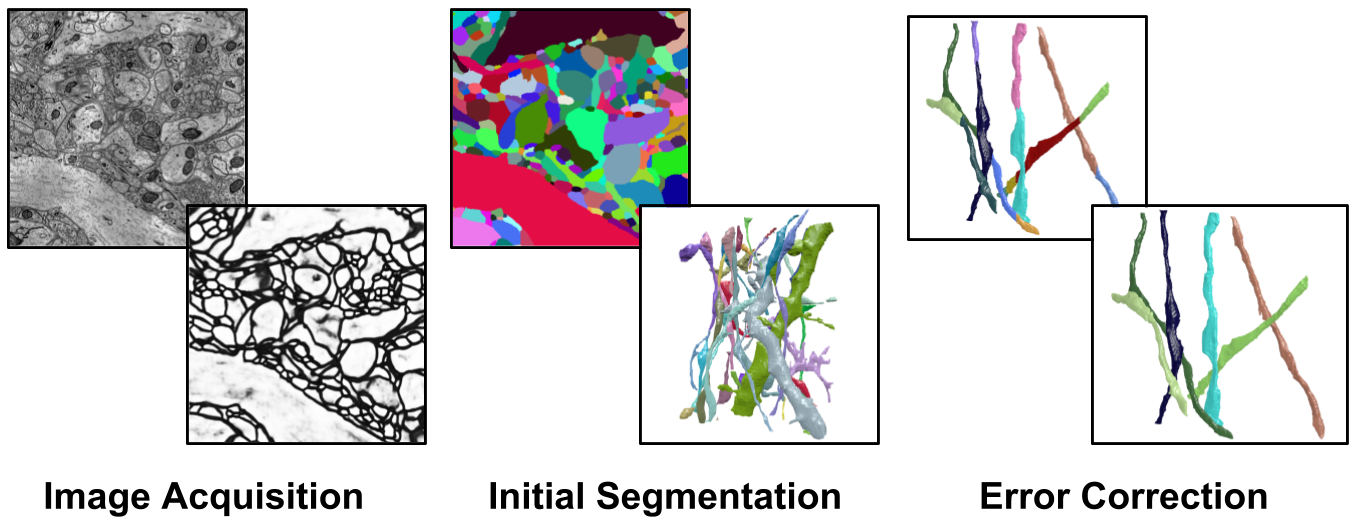
\includegraphics[width=\linewidth]{./figures/proposal-header.png}
	\caption{From an EM image stack, 3D convolutional neural networks generate affinities between voxels (left). A watershed algorithm agglomerates the voxels into supervoxels using these affinities, and these supervoxels are further merged to form a complete segmentation (center). These methods often produce errors and require error correction algorithms to improve the accuracy (right).}
	\label{fig:overview}
\end{figure}


Automatic reconstruction techniques need to be fast, scalable, and accurate.
Ideally, image acquisition is the bottleneck of the connectomics pipeline so reconstruction should occur at a rate of one terabyte per hour~\cite{haehn2017scalable}.
We can achieve this throughput with parallelization among several GPUs with existing techniques~\cite{funke2017deep,parag2017anisotropic}.
However, these automatic methods typically rely on local context for decision making and are agnostic about the underlying biological systems.
Thus, they often make errors at scale and currently require human proofreading or other error correction techniques~\cite{haehn2017guided,error_correction_using_CNN}. 

We propose a novel region merging framework that takes as input an oversegmentation of an EM image stack (under review, \textit{ECCV 2018}).
Our method imposes both local and global biological constraints onto the output segmentation to more closely match the underlying structure of neuronal processes.
Additionally, our method is independent of image resolution and acquisition parameters, enabling its application to isotropic and anisotropic datasets without retraining.
Images generated by electron microscopes often differ in appearance because of variations in staining techniques~\cite{briggman2012volume}.
By removing the dependence of our algorithm on the input images, we greatly reduce the need for additional costly ground truth data for each new stack of images.
